\subsection{Building blocks}%
\label{BuildingBlocks}

\NewScheme{\ANOBE}{ANOBE}
\NewScheme{\DeBE}{DeBE}
\NewAlgorithm{\DeBEsetup}{\DeBE[Setup]}
\NewAlgorithm{\DeBEjoin}{\DeBE[Join]}
\NewAlgorithm{\DeBEenc}{\DeBE[Enc]}
\NewAlgorithm{\DeBEdec}{\DeBE[Dec]}

\paragraph*{Hybrid encryption}\label{KEM}

\Iac{HE} scheme is a combination of \iac{PKE} scheme and \iac{SKE} scheme.
The \ac{PKE} scheme is used as \iac{KEM} to encrypt a symmetric key for the 
\ac{SKE} scheme.
Then the \ac{SKE} scheme is used as \iac{DEM} to encrypt the actual data.

Whenever we use \iac{PKE} scheme, we mean to employ it in \iac{HE} scheme.

\paragraph*{\Acl*{BE}}\label{BE}

\begin{figure}[t]
\centering
  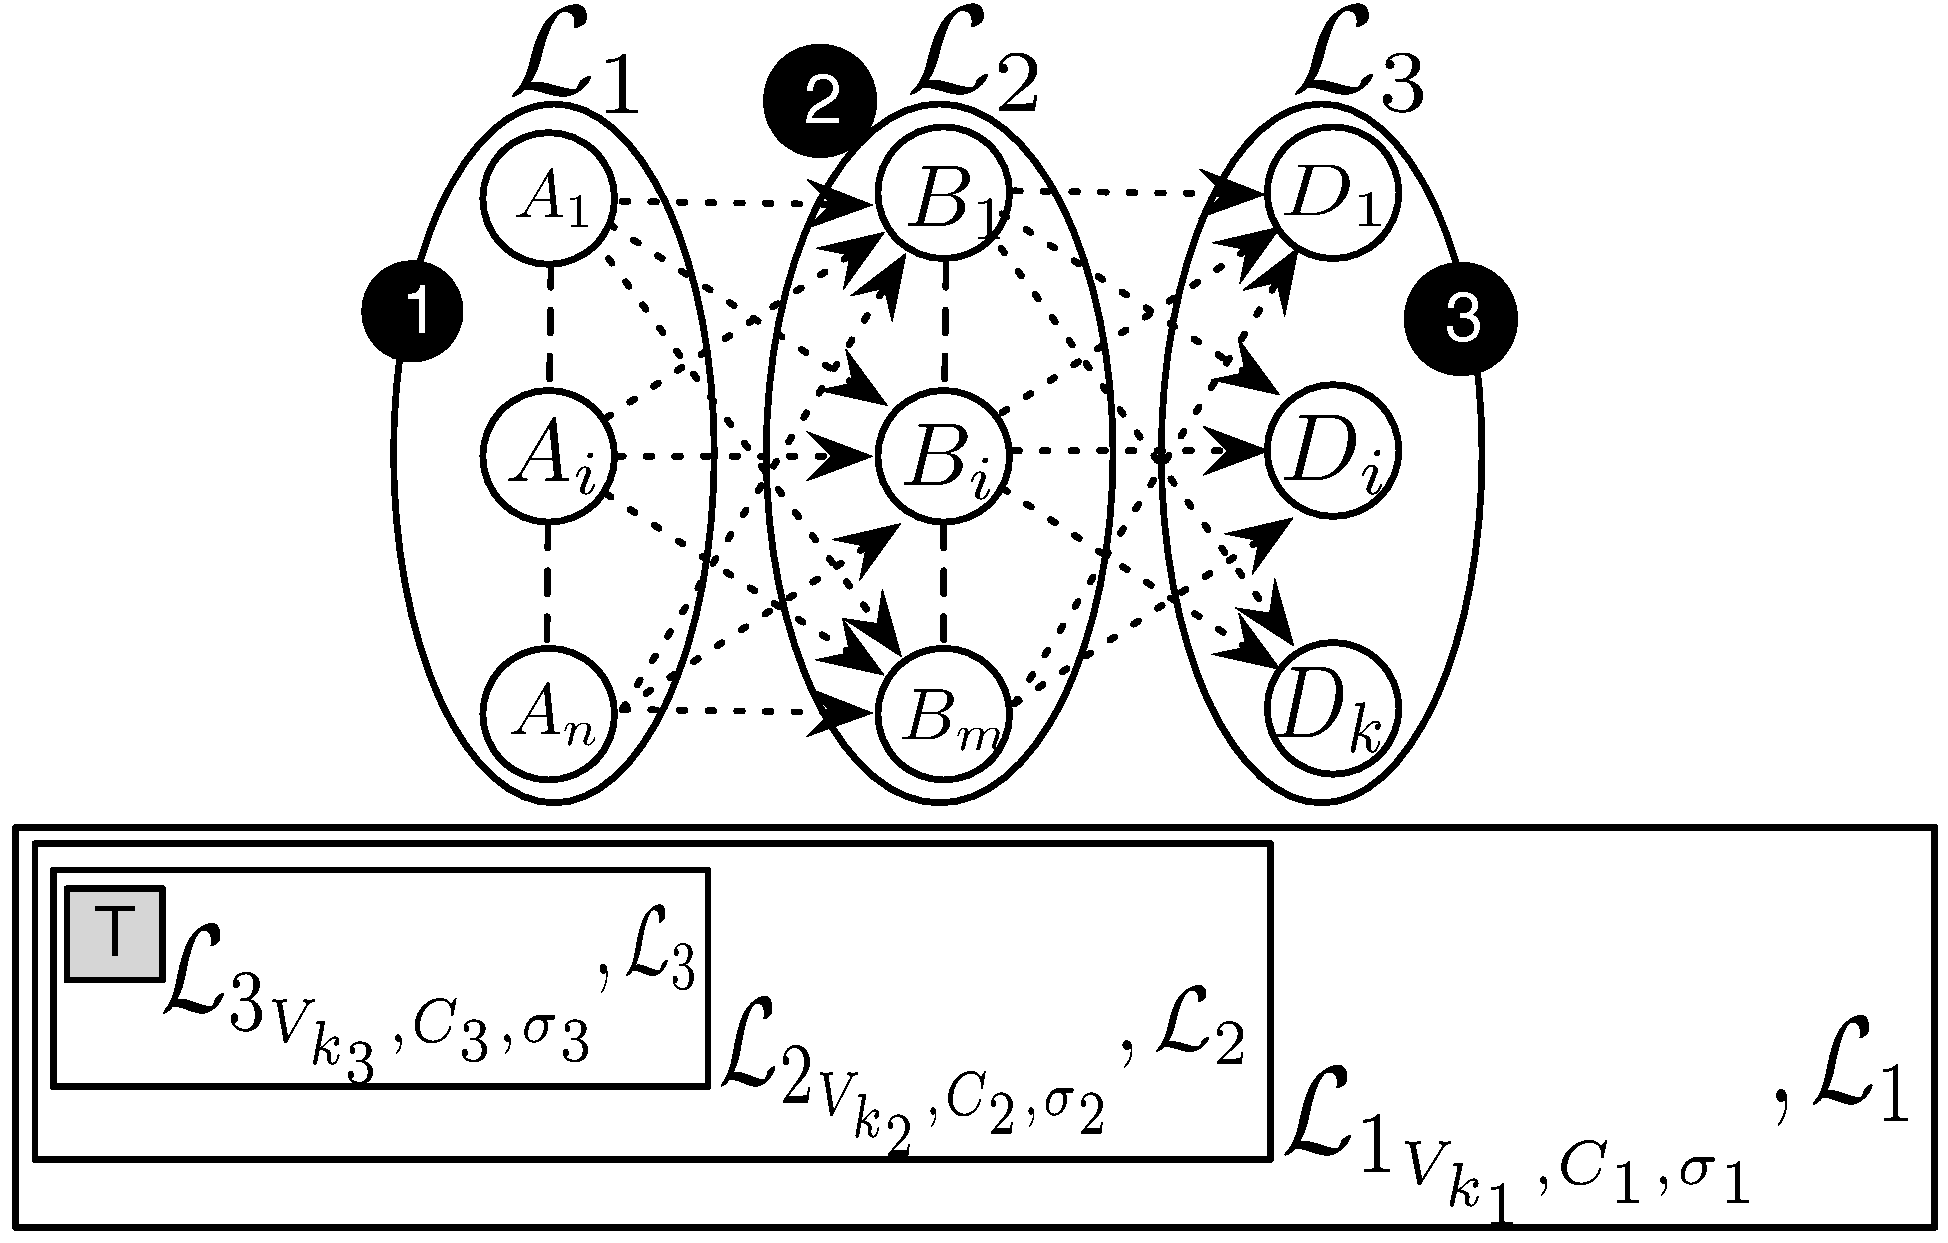
\includegraphics[scale=.20]{figures/pors2.pdf}
  \caption{\label{fig:por} Group Onion Routing}
\end{figure}

in \name, we do onion routing with many
alternative nodes per hop. This means that we encrypt the same message
for more than one possible recipient for each onion layer (See
Figure~\ref{fig:por},\ding{182}, \ding{183}, \ding{184}).
%  Although each node
% has a private and public key, for performances reasons, we want to avoid 
% to encrypt a message multiple times for each onion layer. For instance,
% according to Figure~\ref{fig:por},\ding{182}, \ding{183}, \ding{184},
% we want to avoid to encrypt a
% message $n$ times in layer $\mathcal{L}_1$, $m$ times in layer
% $\mathcal{L}_2$ and $k$ times in layer $\mathcal{L}_3$. 

To encrypt
messages in such a way that only legitimate nodes of a
layer can decrypt them, we leverage on \ac{BE} scheme.
More specifically, we are interested in \iac{BE} scheme adapted to \iac{P2P} 
setting, where devices can dynamically join and leave --- \ie we do not want too 
much cost for joining or leaving, \eg from key regeneration. 
In \name, we require something similar to \iac{DBE} scheme
\cite{DynamicBroadcastEncryption}.
However, we want a slightly different definition.
We say that \iac{BE} scheme is \iac{DeBE} if
\begin{enumerate}
  \item the setup is independent from the expected number of users or an upper 
    bound thereof,
  \item a new user can join at any time and the already issued decryption keys 
    can remain the same,
  \item the previous (public) encryption key can still be used if the newly 
    joined user is not in the recipient set.
\end{enumerate}

% Unlike the definition of \textcite{DynamicBroadcastEncryption}, we desire 
% forward secrecy --- in our scenario it makes no sense that new devices can 
% decrypt old ciphertexts.
% We also want to change the restriction on the ciphertext size:
% whereas \textcite{DynamicBroadcastEncryption} require the ciphertext size to be 
% independent from the expected number of users, we want it to be independent of 
% the total number of users --- \ie it can depend on the recipient set.

% In this sense, the trivial \ac{BE} scheme would fulfil our definition, but not 
% the definition of dynamic~\cite{DynamicBroadcastEncryption}.

To this end, we use the proposed instantiation of \iac{ANOBE} scheme 
to instantiate our own scheme, named \ac{DeBE}. 
In \ac{DeBE}, we simply divide the
steps of the \(\ANOBE\) algorithms differently to suit our
aforementioned requirements. Nevertheless, we are reusing 
both the encryption and decryption algorithms from \cite{ANOBE} to 
encrypt messages which can only be decrypted by a predefined group of
nodes. As a result, our \ac{DeBE} scheme provides among others these algorithms:
\(\DeBEenc, \allowbreak \DeBEdec\) as illustrated in
\cref{DeBEenc}\footnote{For lack of space reasons, we do not introduce the other
algorithms of our \ac{DeBE} scheme}. 

\NewVariable{\mpk}{MPK}
\NewScheme{\Enc}{E}
\NewScheme{\Sign}{S}

% \(\DeBEsetup[\lambda]\): takes the security parameter \(\lambda\) and generates 
% the global parameters for the underlying IND-CCA encryption scheme \(\Enc\) and 
% the one-time signature scheme \(\Sign\).
% It also creates a master public key, \(\mpk = \emptyset\).

\NewVariable{\pk}{pk}
\NewVariable{\sk}{sk}

% \((\pk_i, \sk_i)\gets \DeBEjoin[i]\): generates the public--private key-pair 
% \((\pk_i, \sk_i)\) for device \(i\) when it joins.
% It also adds \(\pk_i\) to \(\mpk\).
% See \cref{DeBEsetup} for an algorithmic overview.

% \begin{figure}
%   \framebox{\begin{minipage}{0.96\linewidth}
%   \begin{algorithmic}
%     \Require{$\Enc$ is an IND-CCA \ac{PKE} scheme, $\Sign$ is a one-time 
%       signature scheme.}

%     \Function{\DeBEsetup}{$\lambda$}
%       \State $\Enc[Setup](\lambda), \Sign[Setup](\lambda)$
%       \State $\mpk\gets \emptyset$
%     \EndFunction

%     \Function{\DeBEjoin}{$i$}
%       \State $(\pk_i, \sk_i)\gets \Enc[Keygen]$
%       \State $\mpk\gets \mpk\cup \{\pk_i\}$
%       \State \Return $(\pk_i, \sk_i)$
%     \EndFunction
%   \end{algorithmic}
%   \end{minipage}}
%   \caption{\label{DeBEsetup}\label{DeBEjoin}%
%     Algorithmic overview of \(\DeBEsetup\) and \(\DeBEjoin\).
%   }
% \end{figure}

\NewVariable{\ssk}{ssk}
\NewVariable{\vk}{vk}

\((\vk, C, \sigma)\gets \DeBEenc[\mpk, S, D, E, m]\):
takes as input: a message \(m\), a recipient set \(D\),  a one-time signature
scheme \(S\), an IND-CCA \ac{PKE} scheme \(E\), and the public keys
set \(MPK\) that contains the public key of each recipient in the set
\(D\), such as $MPK=\sum_{i=1}^{n} pk_i$. The message $m$ is encrypted 
for each recipient's key, then the resulting tuple is
signed.  Finally,the tuple of all ciphertexts, the
verification key, and signature \footnote{The signature
does not authenticate the sender, it ties the ciphertext together and
is needed for correctness, we refer to~\cite{ANOBE} for  details} is returned.

\(m\gets \DeBEdec[\sk_i, (\vk, C, \sigma)]\):
takes a ciphertext \((\vk, C, \sigma)\) and tries to decrypt the sub-ciphertexts 
in \(C\) using the private key \(\sk_i\).
If one succeeds, that message is returned, otherwise \(\bot\) is returned on 
failure.
This trial-and-error decryption is costly as it makes the decryption function 
complexity \(O(|S|)\).
\textcite{ANOBE} also presented a tag-hint system along with their \ac{ANOBE} 
scheme.
The tag-hint system reduced the complexity back to \(O(1)\).
As this is not relevant for our discussion, we refer the reader to~\cite{ANOBE} 
but note that it can be used.

\begin{figure}
  \framebox{\begin{minipage}{0.96\linewidth}
  \begin{algorithmic}[1]
    \Function{$\DeBEenc$}{$\mpk, S, D, E, m$}
      \State $(\ssk, \vk)\gets \Sign[Keygen]$
      \State Choose a random permutation \(\pi\colon D\to D\).
      \For{$i \in D$}
        \State $c_i\gets \Enc[Enc](\pk_i, m\concat \vk)$
      \EndFor
      \State $C\gets ( c_{\pi(1)}, \dotsc, c_{\pi(|S|)} )$
      \State $\sigma\gets \Sign[Sign](\ssk, C)$
      \State \Return $(\vk, C, \sigma)$
    \EndFunction

    \Function{$\DeBEdec$}{$\mpk, \sk_i, (\vk, C, \sigma)$}
      \If{$\Sign[Verify](\vk, C, \sigma) = \bot$}
        \State \Return $\bot$
      \EndIf
      \For{$c\in C$}
        \Comment Trial-and-error decryption
        \State $M\gets{\Enc[Dec](\sk_i, c)}$
        \If{$M = \bot$}
          \State \Return $\bot$
        \ElsIf{$M = (m, \vk)$}
          \State \Return $m$
        \EndIf
      \EndFor
      \State \Return $\bot$
    \EndFunction
  \end{algorithmic}
  \end{minipage}}
  \caption{\label{DeBEenc}\label{DeBEdec}%
    An algorithmic overview of the encryption and decryption algorithms in the 
    \(\DeBE\) scheme, identical to those of \(\ANOBE\).%
  }
\end{figure}

